
% Default to the notebook output style

    


% Inherit from the specified cell style.




    
\documentclass[11pt]{article}

    
    
    \usepackage[T1]{fontenc}
    % Nicer default font (+ math font) than Computer Modern for most use cases
    \usepackage{mathpazo}

    % Basic figure setup, for now with no caption control since it's done
    % automatically by Pandoc (which extracts ![](path) syntax from Markdown).
    \usepackage{graphicx}
    % We will generate all images so they have a width \maxwidth. This means
    % that they will get their normal width if they fit onto the page, but
    % are scaled down if they would overflow the margins.
    \makeatletter
    \def\maxwidth{\ifdim\Gin@nat@width>\linewidth\linewidth
    \else\Gin@nat@width\fi}
    \makeatother
    \let\Oldincludegraphics\includegraphics
    % Set max figure width to be 80% of text width, for now hardcoded.
    \renewcommand{\includegraphics}[1]{\Oldincludegraphics[width=.8\maxwidth]{#1}}
    % Ensure that by default, figures have no caption (until we provide a
    % proper Figure object with a Caption API and a way to capture that
    % in the conversion process - todo).
    \usepackage{caption}
    \DeclareCaptionLabelFormat{nolabel}{}
    \captionsetup{labelformat=nolabel}

    \usepackage{adjustbox} % Used to constrain images to a maximum size 
    \usepackage{xcolor} % Allow colors to be defined
    \usepackage{enumerate} % Needed for markdown enumerations to work
    \usepackage{geometry} % Used to adjust the document margins
    \usepackage{amsmath} % Equations
    \usepackage{amssymb} % Equations
    \usepackage{textcomp} % defines textquotesingle
    % Hack from http://tex.stackexchange.com/a/47451/13684:
    \AtBeginDocument{%
        \def\PYZsq{\textquotesingle}% Upright quotes in Pygmentized code
    }
    \usepackage{upquote} % Upright quotes for verbatim code
    \usepackage{eurosym} % defines \euro
    \usepackage[mathletters]{ucs} % Extended unicode (utf-8) support
    \usepackage[utf8x]{inputenc} % Allow utf-8 characters in the tex document
    \usepackage{fancyvrb} % verbatim replacement that allows latex
    \usepackage{grffile} % extends the file name processing of package graphics 
                         % to support a larger range 
    % The hyperref package gives us a pdf with properly built
    % internal navigation ('pdf bookmarks' for the table of contents,
    % internal cross-reference links, web links for URLs, etc.)
    \usepackage{hyperref}
    \usepackage{longtable} % longtable support required by pandoc >1.10
    \usepackage{booktabs}  % table support for pandoc > 1.12.2
    \usepackage[inline]{enumitem} % IRkernel/repr support (it uses the enumerate* environment)
    \usepackage[normalem]{ulem} % ulem is needed to support strikethroughs (\sout)
                                % normalem makes italics be italics, not underlines
    

    
    
    % Colors for the hyperref package
    \definecolor{urlcolor}{rgb}{0,.145,.698}
    \definecolor{linkcolor}{rgb}{.71,0.21,0.01}
    \definecolor{citecolor}{rgb}{.12,.54,.11}

    % ANSI colors
    \definecolor{ansi-black}{HTML}{3E424D}
    \definecolor{ansi-black-intense}{HTML}{282C36}
    \definecolor{ansi-red}{HTML}{E75C58}
    \definecolor{ansi-red-intense}{HTML}{B22B31}
    \definecolor{ansi-green}{HTML}{00A250}
    \definecolor{ansi-green-intense}{HTML}{007427}
    \definecolor{ansi-yellow}{HTML}{DDB62B}
    \definecolor{ansi-yellow-intense}{HTML}{B27D12}
    \definecolor{ansi-blue}{HTML}{208FFB}
    \definecolor{ansi-blue-intense}{HTML}{0065CA}
    \definecolor{ansi-magenta}{HTML}{D160C4}
    \definecolor{ansi-magenta-intense}{HTML}{A03196}
    \definecolor{ansi-cyan}{HTML}{60C6C8}
    \definecolor{ansi-cyan-intense}{HTML}{258F8F}
    \definecolor{ansi-white}{HTML}{C5C1B4}
    \definecolor{ansi-white-intense}{HTML}{A1A6B2}

    % commands and environments needed by pandoc snippets
    % extracted from the output of `pandoc -s`
    \providecommand{\tightlist}{%
      \setlength{\itemsep}{0pt}\setlength{\parskip}{0pt}}
    \DefineVerbatimEnvironment{Highlighting}{Verbatim}{commandchars=\\\{\}}
    % Add ',fontsize=\small' for more characters per line
    \newenvironment{Shaded}{}{}
    \newcommand{\KeywordTok}[1]{\textcolor[rgb]{0.00,0.44,0.13}{\textbf{{#1}}}}
    \newcommand{\DataTypeTok}[1]{\textcolor[rgb]{0.56,0.13,0.00}{{#1}}}
    \newcommand{\DecValTok}[1]{\textcolor[rgb]{0.25,0.63,0.44}{{#1}}}
    \newcommand{\BaseNTok}[1]{\textcolor[rgb]{0.25,0.63,0.44}{{#1}}}
    \newcommand{\FloatTok}[1]{\textcolor[rgb]{0.25,0.63,0.44}{{#1}}}
    \newcommand{\CharTok}[1]{\textcolor[rgb]{0.25,0.44,0.63}{{#1}}}
    \newcommand{\StringTok}[1]{\textcolor[rgb]{0.25,0.44,0.63}{{#1}}}
    \newcommand{\CommentTok}[1]{\textcolor[rgb]{0.38,0.63,0.69}{\textit{{#1}}}}
    \newcommand{\OtherTok}[1]{\textcolor[rgb]{0.00,0.44,0.13}{{#1}}}
    \newcommand{\AlertTok}[1]{\textcolor[rgb]{1.00,0.00,0.00}{\textbf{{#1}}}}
    \newcommand{\FunctionTok}[1]{\textcolor[rgb]{0.02,0.16,0.49}{{#1}}}
    \newcommand{\RegionMarkerTok}[1]{{#1}}
    \newcommand{\ErrorTok}[1]{\textcolor[rgb]{1.00,0.00,0.00}{\textbf{{#1}}}}
    \newcommand{\NormalTok}[1]{{#1}}
    
    % Additional commands for more recent versions of Pandoc
    \newcommand{\ConstantTok}[1]{\textcolor[rgb]{0.53,0.00,0.00}{{#1}}}
    \newcommand{\SpecialCharTok}[1]{\textcolor[rgb]{0.25,0.44,0.63}{{#1}}}
    \newcommand{\VerbatimStringTok}[1]{\textcolor[rgb]{0.25,0.44,0.63}{{#1}}}
    \newcommand{\SpecialStringTok}[1]{\textcolor[rgb]{0.73,0.40,0.53}{{#1}}}
    \newcommand{\ImportTok}[1]{{#1}}
    \newcommand{\DocumentationTok}[1]{\textcolor[rgb]{0.73,0.13,0.13}{\textit{{#1}}}}
    \newcommand{\AnnotationTok}[1]{\textcolor[rgb]{0.38,0.63,0.69}{\textbf{\textit{{#1}}}}}
    \newcommand{\CommentVarTok}[1]{\textcolor[rgb]{0.38,0.63,0.69}{\textbf{\textit{{#1}}}}}
    \newcommand{\VariableTok}[1]{\textcolor[rgb]{0.10,0.09,0.49}{{#1}}}
    \newcommand{\ControlFlowTok}[1]{\textcolor[rgb]{0.00,0.44,0.13}{\textbf{{#1}}}}
    \newcommand{\OperatorTok}[1]{\textcolor[rgb]{0.40,0.40,0.40}{{#1}}}
    \newcommand{\BuiltInTok}[1]{{#1}}
    \newcommand{\ExtensionTok}[1]{{#1}}
    \newcommand{\PreprocessorTok}[1]{\textcolor[rgb]{0.74,0.48,0.00}{{#1}}}
    \newcommand{\AttributeTok}[1]{\textcolor[rgb]{0.49,0.56,0.16}{{#1}}}
    \newcommand{\InformationTok}[1]{\textcolor[rgb]{0.38,0.63,0.69}{\textbf{\textit{{#1}}}}}
    \newcommand{\WarningTok}[1]{\textcolor[rgb]{0.38,0.63,0.69}{\textbf{\textit{{#1}}}}}
    
    
    % Define a nice break command that doesn't care if a line doesn't already
    % exist.
    \def\br{\hspace*{\fill} \\* }
    % Math Jax compatability definitions
    \def\gt{>}
    \def\lt{<}
    % Document parameters
    \title{documentation}
    
    
    

    % Pygments definitions
    
\makeatletter
\def\PY@reset{\let\PY@it=\relax \let\PY@bf=\relax%
    \let\PY@ul=\relax \let\PY@tc=\relax%
    \let\PY@bc=\relax \let\PY@ff=\relax}
\def\PY@tok#1{\csname PY@tok@#1\endcsname}
\def\PY@toks#1+{\ifx\relax#1\empty\else%
    \PY@tok{#1}\expandafter\PY@toks\fi}
\def\PY@do#1{\PY@bc{\PY@tc{\PY@ul{%
    \PY@it{\PY@bf{\PY@ff{#1}}}}}}}
\def\PY#1#2{\PY@reset\PY@toks#1+\relax+\PY@do{#2}}

\expandafter\def\csname PY@tok@w\endcsname{\def\PY@tc##1{\textcolor[rgb]{0.73,0.73,0.73}{##1}}}
\expandafter\def\csname PY@tok@c\endcsname{\let\PY@it=\textit\def\PY@tc##1{\textcolor[rgb]{0.25,0.50,0.50}{##1}}}
\expandafter\def\csname PY@tok@cp\endcsname{\def\PY@tc##1{\textcolor[rgb]{0.74,0.48,0.00}{##1}}}
\expandafter\def\csname PY@tok@k\endcsname{\let\PY@bf=\textbf\def\PY@tc##1{\textcolor[rgb]{0.00,0.50,0.00}{##1}}}
\expandafter\def\csname PY@tok@kp\endcsname{\def\PY@tc##1{\textcolor[rgb]{0.00,0.50,0.00}{##1}}}
\expandafter\def\csname PY@tok@kt\endcsname{\def\PY@tc##1{\textcolor[rgb]{0.69,0.00,0.25}{##1}}}
\expandafter\def\csname PY@tok@o\endcsname{\def\PY@tc##1{\textcolor[rgb]{0.40,0.40,0.40}{##1}}}
\expandafter\def\csname PY@tok@ow\endcsname{\let\PY@bf=\textbf\def\PY@tc##1{\textcolor[rgb]{0.67,0.13,1.00}{##1}}}
\expandafter\def\csname PY@tok@nb\endcsname{\def\PY@tc##1{\textcolor[rgb]{0.00,0.50,0.00}{##1}}}
\expandafter\def\csname PY@tok@nf\endcsname{\def\PY@tc##1{\textcolor[rgb]{0.00,0.00,1.00}{##1}}}
\expandafter\def\csname PY@tok@nc\endcsname{\let\PY@bf=\textbf\def\PY@tc##1{\textcolor[rgb]{0.00,0.00,1.00}{##1}}}
\expandafter\def\csname PY@tok@nn\endcsname{\let\PY@bf=\textbf\def\PY@tc##1{\textcolor[rgb]{0.00,0.00,1.00}{##1}}}
\expandafter\def\csname PY@tok@ne\endcsname{\let\PY@bf=\textbf\def\PY@tc##1{\textcolor[rgb]{0.82,0.25,0.23}{##1}}}
\expandafter\def\csname PY@tok@nv\endcsname{\def\PY@tc##1{\textcolor[rgb]{0.10,0.09,0.49}{##1}}}
\expandafter\def\csname PY@tok@no\endcsname{\def\PY@tc##1{\textcolor[rgb]{0.53,0.00,0.00}{##1}}}
\expandafter\def\csname PY@tok@nl\endcsname{\def\PY@tc##1{\textcolor[rgb]{0.63,0.63,0.00}{##1}}}
\expandafter\def\csname PY@tok@ni\endcsname{\let\PY@bf=\textbf\def\PY@tc##1{\textcolor[rgb]{0.60,0.60,0.60}{##1}}}
\expandafter\def\csname PY@tok@na\endcsname{\def\PY@tc##1{\textcolor[rgb]{0.49,0.56,0.16}{##1}}}
\expandafter\def\csname PY@tok@nt\endcsname{\let\PY@bf=\textbf\def\PY@tc##1{\textcolor[rgb]{0.00,0.50,0.00}{##1}}}
\expandafter\def\csname PY@tok@nd\endcsname{\def\PY@tc##1{\textcolor[rgb]{0.67,0.13,1.00}{##1}}}
\expandafter\def\csname PY@tok@s\endcsname{\def\PY@tc##1{\textcolor[rgb]{0.73,0.13,0.13}{##1}}}
\expandafter\def\csname PY@tok@sd\endcsname{\let\PY@it=\textit\def\PY@tc##1{\textcolor[rgb]{0.73,0.13,0.13}{##1}}}
\expandafter\def\csname PY@tok@si\endcsname{\let\PY@bf=\textbf\def\PY@tc##1{\textcolor[rgb]{0.73,0.40,0.53}{##1}}}
\expandafter\def\csname PY@tok@se\endcsname{\let\PY@bf=\textbf\def\PY@tc##1{\textcolor[rgb]{0.73,0.40,0.13}{##1}}}
\expandafter\def\csname PY@tok@sr\endcsname{\def\PY@tc##1{\textcolor[rgb]{0.73,0.40,0.53}{##1}}}
\expandafter\def\csname PY@tok@ss\endcsname{\def\PY@tc##1{\textcolor[rgb]{0.10,0.09,0.49}{##1}}}
\expandafter\def\csname PY@tok@sx\endcsname{\def\PY@tc##1{\textcolor[rgb]{0.00,0.50,0.00}{##1}}}
\expandafter\def\csname PY@tok@m\endcsname{\def\PY@tc##1{\textcolor[rgb]{0.40,0.40,0.40}{##1}}}
\expandafter\def\csname PY@tok@gh\endcsname{\let\PY@bf=\textbf\def\PY@tc##1{\textcolor[rgb]{0.00,0.00,0.50}{##1}}}
\expandafter\def\csname PY@tok@gu\endcsname{\let\PY@bf=\textbf\def\PY@tc##1{\textcolor[rgb]{0.50,0.00,0.50}{##1}}}
\expandafter\def\csname PY@tok@gd\endcsname{\def\PY@tc##1{\textcolor[rgb]{0.63,0.00,0.00}{##1}}}
\expandafter\def\csname PY@tok@gi\endcsname{\def\PY@tc##1{\textcolor[rgb]{0.00,0.63,0.00}{##1}}}
\expandafter\def\csname PY@tok@gr\endcsname{\def\PY@tc##1{\textcolor[rgb]{1.00,0.00,0.00}{##1}}}
\expandafter\def\csname PY@tok@ge\endcsname{\let\PY@it=\textit}
\expandafter\def\csname PY@tok@gs\endcsname{\let\PY@bf=\textbf}
\expandafter\def\csname PY@tok@gp\endcsname{\let\PY@bf=\textbf\def\PY@tc##1{\textcolor[rgb]{0.00,0.00,0.50}{##1}}}
\expandafter\def\csname PY@tok@go\endcsname{\def\PY@tc##1{\textcolor[rgb]{0.53,0.53,0.53}{##1}}}
\expandafter\def\csname PY@tok@gt\endcsname{\def\PY@tc##1{\textcolor[rgb]{0.00,0.27,0.87}{##1}}}
\expandafter\def\csname PY@tok@err\endcsname{\def\PY@bc##1{\setlength{\fboxsep}{0pt}\fcolorbox[rgb]{1.00,0.00,0.00}{1,1,1}{\strut ##1}}}
\expandafter\def\csname PY@tok@kc\endcsname{\let\PY@bf=\textbf\def\PY@tc##1{\textcolor[rgb]{0.00,0.50,0.00}{##1}}}
\expandafter\def\csname PY@tok@kd\endcsname{\let\PY@bf=\textbf\def\PY@tc##1{\textcolor[rgb]{0.00,0.50,0.00}{##1}}}
\expandafter\def\csname PY@tok@kn\endcsname{\let\PY@bf=\textbf\def\PY@tc##1{\textcolor[rgb]{0.00,0.50,0.00}{##1}}}
\expandafter\def\csname PY@tok@kr\endcsname{\let\PY@bf=\textbf\def\PY@tc##1{\textcolor[rgb]{0.00,0.50,0.00}{##1}}}
\expandafter\def\csname PY@tok@bp\endcsname{\def\PY@tc##1{\textcolor[rgb]{0.00,0.50,0.00}{##1}}}
\expandafter\def\csname PY@tok@fm\endcsname{\def\PY@tc##1{\textcolor[rgb]{0.00,0.00,1.00}{##1}}}
\expandafter\def\csname PY@tok@vc\endcsname{\def\PY@tc##1{\textcolor[rgb]{0.10,0.09,0.49}{##1}}}
\expandafter\def\csname PY@tok@vg\endcsname{\def\PY@tc##1{\textcolor[rgb]{0.10,0.09,0.49}{##1}}}
\expandafter\def\csname PY@tok@vi\endcsname{\def\PY@tc##1{\textcolor[rgb]{0.10,0.09,0.49}{##1}}}
\expandafter\def\csname PY@tok@vm\endcsname{\def\PY@tc##1{\textcolor[rgb]{0.10,0.09,0.49}{##1}}}
\expandafter\def\csname PY@tok@sa\endcsname{\def\PY@tc##1{\textcolor[rgb]{0.73,0.13,0.13}{##1}}}
\expandafter\def\csname PY@tok@sb\endcsname{\def\PY@tc##1{\textcolor[rgb]{0.73,0.13,0.13}{##1}}}
\expandafter\def\csname PY@tok@sc\endcsname{\def\PY@tc##1{\textcolor[rgb]{0.73,0.13,0.13}{##1}}}
\expandafter\def\csname PY@tok@dl\endcsname{\def\PY@tc##1{\textcolor[rgb]{0.73,0.13,0.13}{##1}}}
\expandafter\def\csname PY@tok@s2\endcsname{\def\PY@tc##1{\textcolor[rgb]{0.73,0.13,0.13}{##1}}}
\expandafter\def\csname PY@tok@sh\endcsname{\def\PY@tc##1{\textcolor[rgb]{0.73,0.13,0.13}{##1}}}
\expandafter\def\csname PY@tok@s1\endcsname{\def\PY@tc##1{\textcolor[rgb]{0.73,0.13,0.13}{##1}}}
\expandafter\def\csname PY@tok@mb\endcsname{\def\PY@tc##1{\textcolor[rgb]{0.40,0.40,0.40}{##1}}}
\expandafter\def\csname PY@tok@mf\endcsname{\def\PY@tc##1{\textcolor[rgb]{0.40,0.40,0.40}{##1}}}
\expandafter\def\csname PY@tok@mh\endcsname{\def\PY@tc##1{\textcolor[rgb]{0.40,0.40,0.40}{##1}}}
\expandafter\def\csname PY@tok@mi\endcsname{\def\PY@tc##1{\textcolor[rgb]{0.40,0.40,0.40}{##1}}}
\expandafter\def\csname PY@tok@il\endcsname{\def\PY@tc##1{\textcolor[rgb]{0.40,0.40,0.40}{##1}}}
\expandafter\def\csname PY@tok@mo\endcsname{\def\PY@tc##1{\textcolor[rgb]{0.40,0.40,0.40}{##1}}}
\expandafter\def\csname PY@tok@ch\endcsname{\let\PY@it=\textit\def\PY@tc##1{\textcolor[rgb]{0.25,0.50,0.50}{##1}}}
\expandafter\def\csname PY@tok@cm\endcsname{\let\PY@it=\textit\def\PY@tc##1{\textcolor[rgb]{0.25,0.50,0.50}{##1}}}
\expandafter\def\csname PY@tok@cpf\endcsname{\let\PY@it=\textit\def\PY@tc##1{\textcolor[rgb]{0.25,0.50,0.50}{##1}}}
\expandafter\def\csname PY@tok@c1\endcsname{\let\PY@it=\textit\def\PY@tc##1{\textcolor[rgb]{0.25,0.50,0.50}{##1}}}
\expandafter\def\csname PY@tok@cs\endcsname{\let\PY@it=\textit\def\PY@tc##1{\textcolor[rgb]{0.25,0.50,0.50}{##1}}}

\def\PYZbs{\char`\\}
\def\PYZus{\char`\_}
\def\PYZob{\char`\{}
\def\PYZcb{\char`\}}
\def\PYZca{\char`\^}
\def\PYZam{\char`\&}
\def\PYZlt{\char`\<}
\def\PYZgt{\char`\>}
\def\PYZsh{\char`\#}
\def\PYZpc{\char`\%}
\def\PYZdl{\char`\$}
\def\PYZhy{\char`\-}
\def\PYZsq{\char`\'}
\def\PYZdq{\char`\"}
\def\PYZti{\char`\~}
% for compatibility with earlier versions
\def\PYZat{@}
\def\PYZlb{[}
\def\PYZrb{]}
\makeatother


    % Exact colors from NB
    \definecolor{incolor}{rgb}{0.0, 0.0, 0.5}
    \definecolor{outcolor}{rgb}{0.545, 0.0, 0.0}



    
    % Prevent overflowing lines due to hard-to-break entities
    \sloppy 
    % Setup hyperref package
    \hypersetup{
      breaklinks=true,  % so long urls are correctly broken across lines
      colorlinks=true,
      urlcolor=urlcolor,
      linkcolor=linkcolor,
      citecolor=citecolor,
      }
    % Slightly bigger margins than the latex defaults
    
    \geometry{verbose,tmargin=1in,bmargin=1in,lmargin=1in,rmargin=1in}
    
    

    \begin{document}
    
    
    \maketitle
    
    

    
    \section{Datenbanksysteme (SoSe22)
Project}\label{datenbanksysteme-sose22-project}

Yvette Hung, Haoyang Zhou, Maximilian Krügerke

    \subsection{Project idea}\label{project-idea}

After finding the source of the given dataset, we know that it contains
data of a literature review on a specific topic. If someone were to
conduct research on this topic, this dataset would be useful for finding
past studies. To make their citations more reliable, we found a second
dataset containing impact factor data on various scientific journals.
When compared with the literature review dataset, it enables users to
identify which articles are published in authoritative journals. We
assume that there is a positive correlation between a journal's impact
factor and its reliability.

In our database, each of the two datasets is represented by a table.

    \subsection{Datasets used}\label{datasets-used}

\begin{itemize}
\tightlist
\item
  Given dataset:
  https://tudatalib.ulb.tu-darmstadt.de/handle/tudatalib/2478
\item
  Second dataset from
  https://www.kaggle.com/datasets/mostafafaramin/scientific-journals-ranking-sjr.
  This dataset ranks scientific journals based on their impact factor
  (IF) in 2020.
\end{itemize}

    Below we visualize the two datasets as tables:

    \begin{Verbatim}[commandchars=\\\{\}]
{\color{incolor}In [{\color{incolor}1}]:} \PY{k+kn}{import} \PY{n+nn}{pandas} \PY{k}{as} \PY{n+nn}{pd}
\end{Verbatim}


    \begin{Verbatim}[commandchars=\\\{\}]
{\color{incolor}In [{\color{incolor}2}]:} \PY{c+c1}{\PYZsh{} given dataset}
        \PY{n}{lit\PYZus{}df} \PY{o}{=} \PY{n}{pd}\PY{o}{.}\PY{n}{read\PYZus{}csv}\PY{p}{(}\PY{l+s+s1}{\PYZsq{}}\PY{l+s+s1}{Literature\PYZhy{}data\PYZus{}TU\PYZhy{}Darmstadt.txt}\PY{l+s+s1}{\PYZsq{}}\PY{p}{,} \PY{n}{sep} \PY{o}{=} \PY{l+s+s1}{\PYZsq{}}\PY{l+s+se}{\PYZbs{}t}\PY{l+s+s1}{\PYZsq{}}\PY{p}{,} \PY{n}{header} \PY{o}{=} \PY{l+m+mi}{1}\PY{p}{,} \PY{n}{skiprows} \PY{o}{=} \PY{p}{[}\PY{l+m+mi}{3}\PY{p}{]}\PY{p}{)}
        \PY{n}{lit\PYZus{}df}\PY{o}{.}\PY{n}{head}\PY{p}{(}\PY{l+m+mi}{5}\PY{p}{)}
\end{Verbatim}


\begin{Verbatim}[commandchars=\\\{\}]
{\color{outcolor}Out[{\color{outcolor}2}]:}   Quelle                                              Autor  \textbackslash{}
        0    WOS  Chaudhary, Ayesha Hoor; Bukhari, Faisal; Iqbal{\ldots}   
        1    WOS  Kim, Soo-Kyun; Lee, Chang-Hee; Kim, Sun-Jeong;{\ldots}   
        2    WOS                     Lee, Byong Kwon; Lee, Yang Sun   
        3    WOS  Frederiksen, Joakim Grant; Sorensen, Stine May{\ldots}   
        4    WOS      Rafique, Muhammad Usman; Cheung, Sen-ching S.   
        
                                                       Titel  Jahr  \textbackslash{}
        0     Laparoscopic Training Exercises Using HTC VIVE  2020   
        1  Implementation of Local Area VR Environment us{\ldots}  2020   
        2  Distinction Between Real Faces and Photos by A{\ldots}  2020   
        3  Cognitive load and performance in immersive vi{\ldots}  2020   
        4        Tracking Attacks on Virtual Reality Systems  2020   
        
                                                     Journal  Typ  \textbackslash{}
        0          INTELLIGENT AUTOMATION AND SOFT COMPUTING  NaN   
        1          INTELLIGENT AUTOMATION AND SOFT COMPUTING  NaN   
        2          INTELLIGENT AUTOMATION AND SOFT COMPUTING  NaN   
        3  SURGICAL ENDOSCOPY AND OTHER INTERVENTIONAL TE{\ldots}  NaN   
        4                 IEEE CONSUMER ELECTRONICS MAGAZINE  NaN   
        
                                  DOI Gelesen? Empirisch? Ausschlusspunkt  {\ldots}   \textbackslash{}
        0     10.31209/2019.100000149    Görge        NaN           Titel  {\ldots}    
        1     10.31209/2019.100000131    Görge        NaN           Titel  {\ldots}    
        2     10.31209/2019.100000134    Görge        NaN           Titel  {\ldots}    
        3  10.1007/s00464-019-06887-8    Görge         Ja          Sample  {\ldots}    
        4    10.1109/MCE.2019.2953741    Görge       Nein        Abstract  {\ldots}    
        
          Cognitive / Memory tasks Spatial Perception Quantitative Qualitative  \textbackslash{}
        0                      NaN                NaN          NaN         NaN   
        1                      NaN                NaN          NaN         NaN   
        2                      NaN                NaN          NaN         NaN   
        3                      NaN                  x            x         NaN   
        4                      NaN                NaN          NaN         NaN   
        
          Experiment Secondary research   Subjective feedback Consistent Better Worse  
        0        NaN                 NaN                  NaN        NaN    NaN   NaN  
        1        NaN                 NaN                  NaN        NaN    NaN   NaN  
        2        NaN                 NaN                  NaN        NaN    NaN   NaN  
        3          x                 NaN                  NaN        NaN    NaN     x  
        4        NaN                 NaN                  NaN        NaN    NaN   NaN  
        
        [5 rows x 41 columns]
\end{Verbatim}
            
    \begin{Verbatim}[commandchars=\\\{\}]
{\color{incolor}In [{\color{incolor}3}]:} \PY{c+c1}{\PYZsh{} dataset of journal impact factors}
        \PY{n}{jif\PYZus{}df} \PY{o}{=} \PY{n}{pd}\PY{o}{.}\PY{n}{read\PYZus{}csv}\PY{p}{(}\PY{l+s+s1}{\PYZsq{}}\PY{l+s+s1}{journal\PYZus{}impact\PYZus{}factors\PYZus{}2020.csv}\PY{l+s+s1}{\PYZsq{}}\PY{p}{)}
        \PY{n}{jif\PYZus{}df}\PY{o}{.}\PY{n}{head}\PY{p}{(}\PY{l+m+mi}{5}\PY{p}{)}
\end{Verbatim}


\begin{Verbatim}[commandchars=\\\{\}]
{\color{outcolor}Out[{\color{outcolor}3}]:}    Rank                  Full Journal Title Journal Impact Factor  \textbackslash{}
        0     1  CA-A CANCER JOURNAL FOR CLINICIANS               292.278   
        1     2     NEW ENGLAND JOURNAL OF MEDICINE                74.699   
        2     3            Nature Reviews Materials                71.189   
        3     4       NATURE REVIEWS DRUG DISCOVERY                64.797   
        4     5                              LANCET                60.392   
        
           Impact Factor without Journal Self Cites 5-Year Impact Factor  \textbackslash{}
        0                                   291.481               225.87   
        1                                    73.983               72.098   
        2                                    70.968               84.972   
        3                                    63.905               60.796   
        4                                    59.208               59.345   
        
          Cited Half-Life Citing Half-life \% Articles in Citable Items  \textbackslash{}
        0             3.4              4.6                       77.27   
        1             8.7              4.9                       84.45   
        2             2.8              5.5                        2.27   
        3             8.2              5.5                       11.11   
        4             8.6              4.2                       69.82   
        
          Average Journal Impact Factor Percentile  
        0                                   99.795  
        1                                   99.697  
        2                                   99.678  
        3                                   99.747  
        4                                   99.091  
\end{Verbatim}
            
    \subsection{Data schema}\label{data-schema}

\subsubsection{ERM}\label{erm}

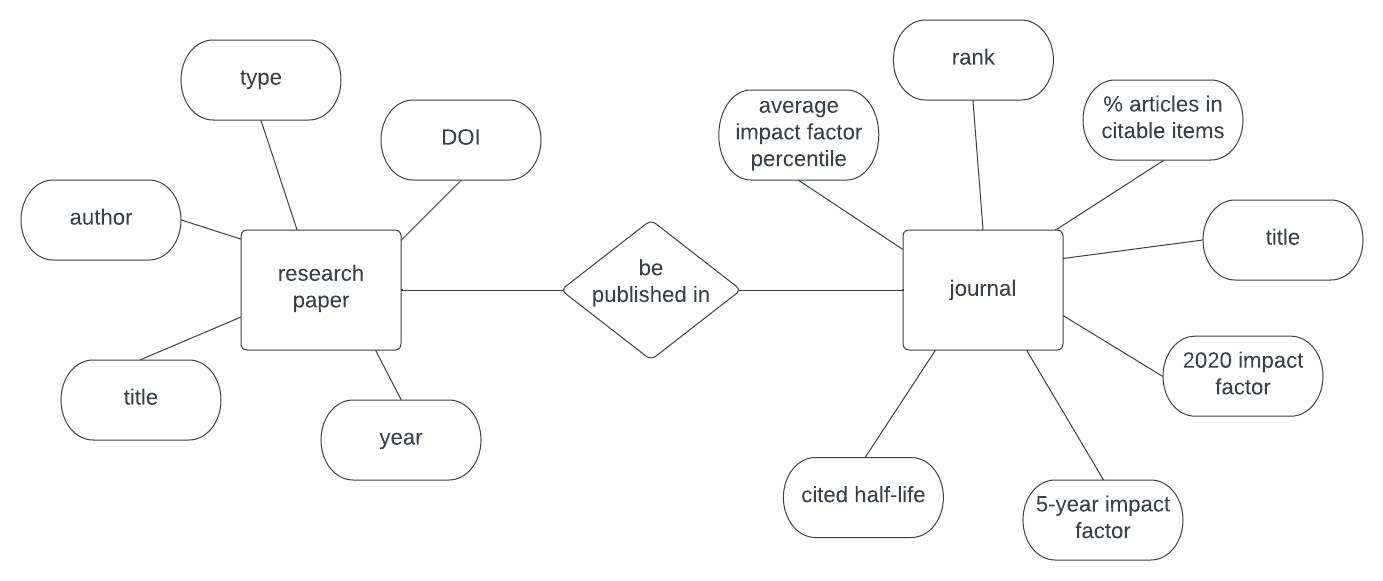
\includegraphics{images/ERM_2.png} \#\#\# Relational model literature
(Titel, Autor, Jahr, Journal, Typ, DOI)\\
journals (Title, Rank, Impact\_Factor, IF\_5\_Yr, Half\_Life,
Percentage\_Citable, Avg\_IF\_Percentile)

    \subsection{Data Pre-processing}\label{data-pre-processing}

\subsubsection{Steps}\label{steps}

\begin{itemize}
\tightlist
\item
  Keep the attributes we need according to our relational model.
\item
  Convert some string columns to lowercase for consistency. For example,
  some journal titles were all capitalized while others were only
  capitalized on the first letter ("BRAIN SCIENCES" vs "Brain
  Sciences").
\item
  Deal with null values
\item
  Literature dataset: identify and remove duplicates (marked with
  Ausschlusspunkt = "Dopplung")
\end{itemize}

The processed datasets we imported to the database are shown below:

    \begin{Verbatim}[commandchars=\\\{\}]
{\color{incolor}In [{\color{incolor}4}]:} \PY{n}{literature\PYZus{}df} \PY{o}{=} \PY{n}{pd}\PY{o}{.}\PY{n}{read\PYZus{}csv}\PY{p}{(}\PY{l+s+s1}{\PYZsq{}}\PY{l+s+s1}{literature\PYZus{}dataset.csv}\PY{l+s+s1}{\PYZsq{}}\PY{p}{)}
        \PY{n}{literature\PYZus{}df}\PY{o}{.}\PY{n}{head}\PY{p}{(}\PY{l+m+mi}{5}\PY{p}{)}
\end{Verbatim}


\begin{Verbatim}[commandchars=\\\{\}]
{\color{outcolor}Out[{\color{outcolor}4}]:}                                                Titel  \textbackslash{}
        0     laparoscopic training exercises using htc vive   
        1  implementation of local area vr environment us{\ldots}   
        2  distinction between real faces and photos by a{\ldots}   
        3  cognitive load and performance in immersive vi{\ldots}   
        4        tracking attacks on virtual reality systems   
        
                                                       Autor  Jahr  \textbackslash{}
        0  chaudhary, ayesha hoor; bukhari, faisal; iqbal{\ldots}  2020   
        1  kim, soo-kyun; lee, chang-hee; kim, sun-jeong;{\ldots}  2020   
        2                     lee, byong kwon; lee, yang sun  2020   
        3  frederiksen, joakim grant; sorensen, stine may{\ldots}  2020   
        4      rafique, muhammad usman; cheung, sen-ching s.  2020   
        
                                                     Journal  Typ  \textbackslash{}
        0          intelligent automation and soft computing  NaN   
        1          intelligent automation and soft computing  NaN   
        2          intelligent automation and soft computing  NaN   
        3  surgical endoscopy and other interventional te{\ldots}  NaN   
        4                 ieee consumer electronics magazine  NaN   
        
                                  DOI  
        0     10.31209/2019.100000149  
        1     10.31209/2019.100000131  
        2     10.31209/2019.100000134  
        3  10.1007/s00464-019-06887-8  
        4    10.1109/MCE.2019.2953741  
\end{Verbatim}
            
    \begin{Verbatim}[commandchars=\\\{\}]
{\color{incolor}In [{\color{incolor}5}]:} \PY{n}{journals\PYZus{}df} \PY{o}{=} \PY{n}{pd}\PY{o}{.}\PY{n}{read\PYZus{}csv}\PY{p}{(}\PY{l+s+s1}{\PYZsq{}}\PY{l+s+s1}{journal\PYZus{}dataset.csv}\PY{l+s+s1}{\PYZsq{}}\PY{p}{)}
        \PY{n}{journals\PYZus{}df}\PY{o}{.}\PY{n}{head}\PY{p}{(}\PY{l+m+mi}{5}\PY{p}{)}
\end{Verbatim}


\begin{Verbatim}[commandchars=\\\{\}]
{\color{outcolor}Out[{\color{outcolor}5}]:}                                 Title  Rank  Impact\_Factor  IF\_5\_Yr  \textbackslash{}
        0  ca-a cancer journal for clinicians     1        292.278  225.870   
        1     new england journal of medicine     2         74.699   72.098   
        2            nature reviews materials     3         71.189   84.972   
        3       nature reviews drug discovery     4         64.797   60.796   
        4                              lancet     5         60.392   59.345   
        
           Half\_Life  Percentage\_Citable  Avg\_IF\_Percentile  
        0        3.4               77.27             99.795  
        1        8.7               84.45             99.697  
        2        2.8                2.27             99.678  
        3        8.2               11.11             99.747  
        4        8.6               69.82             99.091  
\end{Verbatim}
            
    \subsubsection{Challenges}\label{challenges}

\begin{itemize}
\tightlist
\item
  Initially there were some difficulties with importing the given
  dataset because the first few lines caused the columns to be parsed
  incorrectly.
\item
  Even though duplicate rows in the literature dataset were marked,
  there were still differences between them in a few cases, so we had to
  delete the one not marked with "Dopplung". In the image below, the row
  marked with "Dopplung" contains a DOI value, while the other does not.
  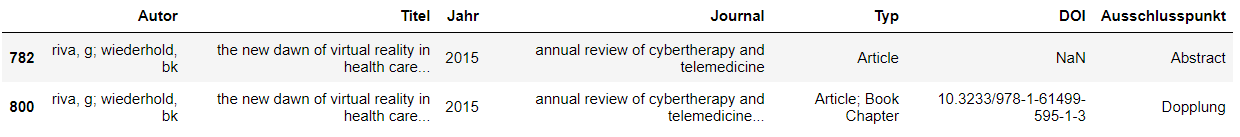
\includegraphics{images/example_duplicate.png}
\item
  We couldn't find duplicates for two rows marked with "Dopplung", so we
  kept them in the dataset.
\item
  Deciding what to do with null values

  \begin{itemize}
  \tightlist
  \item
    Since we are using research paper titles for the index in the
    literature dataset, we decided to replace null values in the DOI
    column with zeroes.
  \item
    Null values in the impact factor dataset were strings ("Not
    Available"). We changed them to NaN instead.
  \end{itemize}
\end{itemize}

    \subsection{Database set up}\label{database-set-up}

\subsubsection{Steps}\label{steps}

\begin{itemize}
\tightlist
\item
  Install PostgreSQL and create a database locally
\item
  Install and import psycopg2
\item
  Open connection to database
\item
  Read in data files and create two tables ("literature" and "journals")
\item
  Close connection when done
\end{itemize}

\subsubsection{Challenges}\label{challenges}

\begin{itemize}
\item
  Since our files are CSVs, the copy\_from function in the given example
  failed to correctly parse values - it didn't ignore commas in quotes,
  which resulted in more columns than there actually were. We tried
  using TSV files instead, but reading in individual lines became more
  difficult because the readline function didn't work in this case. In
  the end we decided on the copy\_expert function:

\begin{Shaded}
\begin{Highlighting}[]
\NormalTok{f1 }\OperatorTok{=} \BuiltInTok{open}\NormalTok{(}\StringTok{'literature_dataset.csv'}\NormalTok{)}
\NormalTok{cur.copy_expert(}\StringTok{"""COPY literature FROM STDIN WITH CSV HEADER DELIMITER AS ','"""}\NormalTok{, f1)}
\end{Highlighting}
\end{Shaded}
\item
  After failing to create tables on the first try, we encountered
  another error on the second try: "DatabaseError: current transaction
  is aborted, commands ignored until end of transaction block". We had
  to roll back the transaction before trying again.
\end{itemize}

    \subsection{Web application}\label{web-application}

\subsubsection{Decisions}\label{decisions}

\begin{itemize}
\item
  For easier and more systematic creation of tables, we defined all
  columns as type \texttt{varchar} according to the given project
  example. This made conditions involving integers (e.g. sorting by
  year) more complicated - we had to explicitly convert those columns to
  type \texttt{INT}.
\item
  For some sorting and filtering functions, multiple options are
  provided for the user to toggle between, for example
  ascending/descending sorting order:

\begin{Shaded}
\begin{Highlighting}[]
\NormalTok{order }\OperatorTok{=} \StringTok{'ASC'}
\CommentTok{# order = 'DESC'}
\end{Highlighting}
\end{Shaded}
\item
  We make it easy to switch between queries by defining them beforehand
  and changing the value of a designated variable used in the execute
  function. For example:

\begin{Shaded}
\begin{Highlighting}[]
\NormalTok{query1 }\OperatorTok{=} \StringTok{"""SELECT * FROM literature"""}
\NormalTok{query2 }\OperatorTok{=} \StringTok{"""SELECT * FROM journals"""}
\NormalTok{sql_query }\OperatorTok{=}\NormalTok{ query1 }\CommentTok{# change the value of this variable}
\NormalTok{cur.execute(sql_query)}
\end{Highlighting}
\end{Shaded}
\end{itemize}

    \subsubsection{Sorting functions}\label{sorting-functions}

\paragraph{Sort by journal ranking}\label{sort-by-journal-ranking}

\begin{itemize}
\tightlist
\item
  Useful when initially searching for papers to read - find research
  articles published by the most impactful journals.
\item
  Ascending/descending order can be changed.
\end{itemize}

SQL query used:

\begin{Shaded}
\begin{Highlighting}[]
\KeywordTok{SELECT}\NormalTok{ L.Titel, Autor, J.Title, }\FunctionTok{CAST}\NormalTok{ (}\FunctionTok{Rank} \KeywordTok{AS} \DataTypeTok{INT}\NormalTok{), Impact_Factor, IF_5_Yr}
\KeywordTok{FROM}\NormalTok{ literature }\KeywordTok{AS}\NormalTok{ L, journals }\KeywordTok{AS}\NormalTok{ J}
\KeywordTok{WHERE}\NormalTok{ L.Journal = J.Title}
\KeywordTok{ORDER} \KeywordTok{BY} \FunctionTok{Rank} \KeywordTok{ASC}\NormalTok{;}
\end{Highlighting}
\end{Shaded}

Next we use the \texttt{read\_sql\_query} function to execute the query
and retrieve the results in a pandas dataframe:

\begin{Shaded}
\begin{Highlighting}[]
\NormalTok{df }\OperatorTok{=}\NormalTok{ pd.read_sql_query(sql_query, conn)}
\end{Highlighting}
\end{Shaded}

The dataframe is displayed as follows:\\
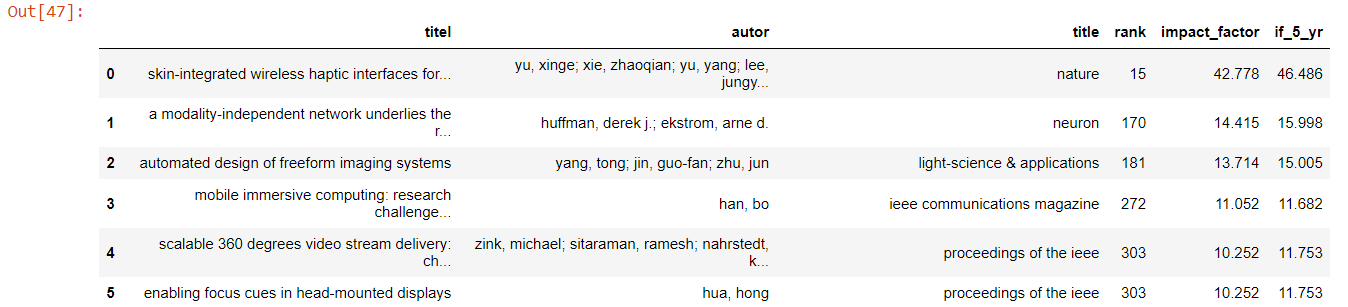
\includegraphics{images/sortrank_df.png}

\paragraph{Sort by publication year}\label{sort-by-publication-year}

\begin{itemize}
\tightlist
\item
  Useful if the user wants to find the newest articles.
\item
  Ascending/descending order can be changed.
\end{itemize}

Example of the SQL query used and its output:

\begin{Shaded}
\begin{Highlighting}[]
\KeywordTok{SELECT}\NormalTok{ L.Titel, Autor, }\FunctionTok{CAST}\NormalTok{ (Jahr }\KeywordTok{AS} \DataTypeTok{INT}\NormalTok{), J.Title, }\FunctionTok{Rank}\NormalTok{, IF_5_Yr}
\KeywordTok{FROM}\NormalTok{ literature }\KeywordTok{AS}\NormalTok{ L, journals }\KeywordTok{AS}\NormalTok{ J}
\KeywordTok{WHERE}\NormalTok{ L.Journal = J.Title}
\KeywordTok{ORDER} \KeywordTok{BY}\NormalTok{ Jahr }\KeywordTok{DESC}\NormalTok{;}
\end{Highlighting}
\end{Shaded}

\begin{figure}
\centering
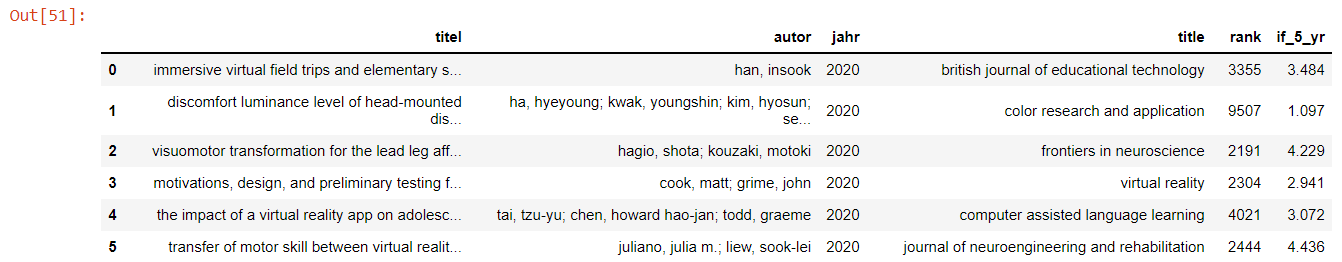
\includegraphics{images/sortyear_df.png}
\caption{results of the sort by year query}
\end{figure}

    \subsubsection{Filter functions}\label{filter-functions}

\paragraph{Filter by publication year}\label{filter-by-publication-year}

\begin{itemize}
\tightlist
\item
  Filter for papers published either before, after, or during a certain
  year.
\item
  Three operator options (\texttt{\textless{}=}, \texttt{=},
  \texttt{\textgreater{}=}) are provided.
\end{itemize}

An example of the SQL query used and its output:

\begin{Shaded}
\begin{Highlighting}[]
\KeywordTok{SELECT}\NormalTok{ L.Titel, Autor, Jahr, J.Title, }\FunctionTok{Rank}\NormalTok{, IF_5_Yr}
\KeywordTok{FROM}\NormalTok{ literature }\KeywordTok{AS}\NormalTok{ L, journals }\KeywordTok{AS}\NormalTok{ J}
\KeywordTok{WHERE}\NormalTok{ L.Journal = J.Title}
\KeywordTok{AND} \FunctionTok{CAST}\NormalTok{ (Jahr }\KeywordTok{AS} \DataTypeTok{INT}\NormalTok{) = }\DecValTok{2018}\NormalTok{;}
\end{Highlighting}
\end{Shaded}

\begin{figure}
\centering
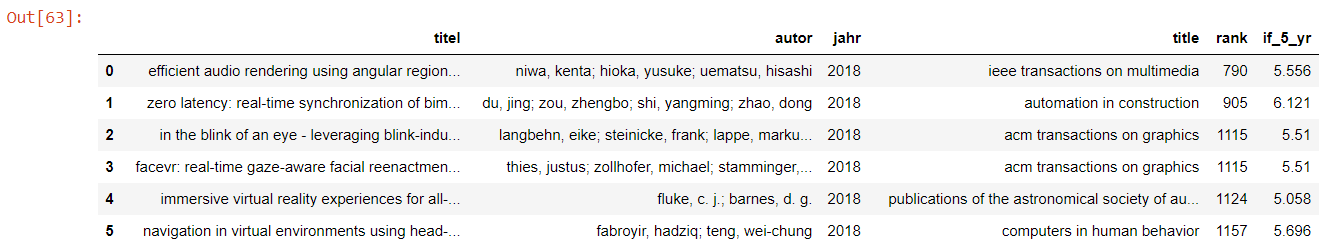
\includegraphics{images/filteryear_df.png}
\caption{results of the filter by year query}
\end{figure}

\paragraph{Filter by author}\label{filter-by-author}

\begin{itemize}
\tightlist
\item
  Useful when the user wants to search for other articles written by an
  author.
\item
  Uses the \texttt{LIKE} operator and \texttt{\%} wildcards because most
  papers are written by multiple authors.
\item
  Works better using last names because some first names are abbreviated
  (e.g. "Riva, G.").
\end{itemize}

Example SQL query and its output:

\begin{Shaded}
\begin{Highlighting}[]
\KeywordTok{SELECT}\NormalTok{ L.Titel, Autor, J.Title, }\FunctionTok{Rank}\NormalTok{, Impact_Factor, IF_5_Yr}
\KeywordTok{FROM}\NormalTok{ literature }\KeywordTok{AS}\NormalTok{ L, journals }\KeywordTok{AS}\NormalTok{ J}
\KeywordTok{WHERE}\NormalTok{ L.Journal = J.Title}
\KeywordTok{AND}\NormalTok{ Autor }\KeywordTok{LIKE} \StringTok{'%steinicke%'}\NormalTok{;}
\end{Highlighting}
\end{Shaded}

\begin{figure}
\centering
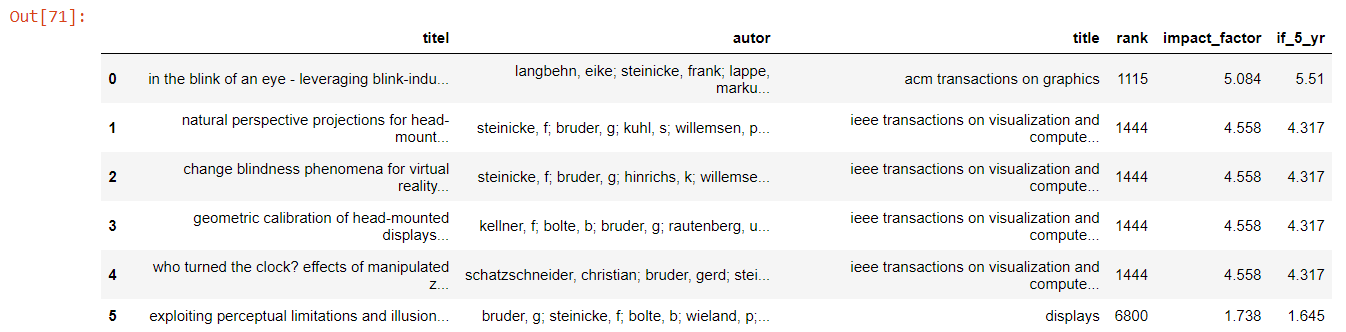
\includegraphics{images/filterauthor_df.png}
\caption{results of the filter by author query}
\end{figure}

\paragraph{Filter by ranking of the publishing
journal}\label{filter-by-ranking-of-the-publishing-journal}

\begin{itemize}
\tightlist
\item
  Find papers published by journals within a certain ranking.
\item
  The specific ranking can be changed.
\end{itemize}

Example SQL query and its output:

\begin{Shaded}
\begin{Highlighting}[]
\KeywordTok{SELECT}\NormalTok{ L.Titel, Autor, Jahr, J.Title, }\FunctionTok{Rank}\NormalTok{, IF_5_Yr}
\KeywordTok{FROM}\NormalTok{ literature }\KeywordTok{AS}\NormalTok{ L, journals }\KeywordTok{AS}\NormalTok{ J}
\KeywordTok{WHERE}\NormalTok{ L.Journal = J.Title}
\KeywordTok{AND} \FunctionTok{CAST}\NormalTok{ (}\FunctionTok{Rank} \KeywordTok{AS} \DataTypeTok{INT}\NormalTok{) <= }\DecValTok{500}\NormalTok{;}
\end{Highlighting}
\end{Shaded}

\begin{figure}
\centering
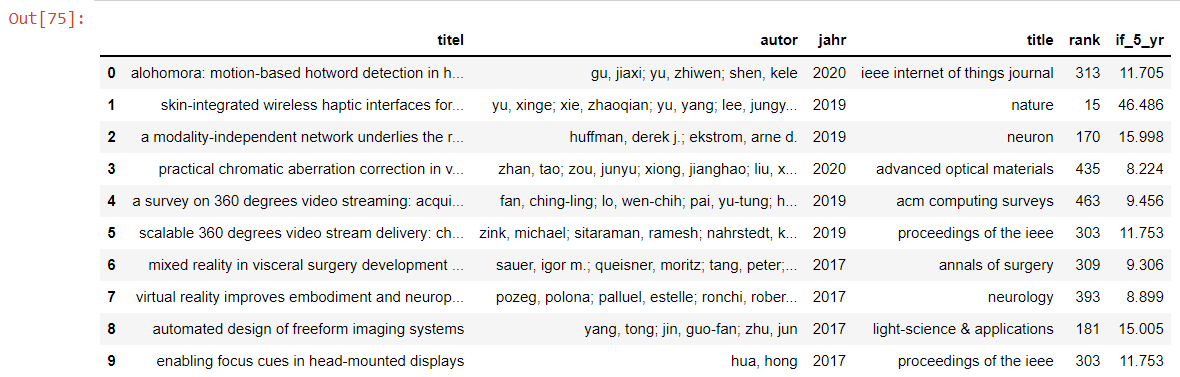
\includegraphics{images/filterrank_df.png}
\caption{results of the filter by rank query}
\end{figure}


    % Add a bibliography block to the postdoc
    
    
    
    \end{document}
